\documentclass[conference]{IEEEtran}

\usepackage{cite}
\usepackage{graphicx}
\usepackage{amsmath,amssymb,amsfonts}
\usepackage{algorithmic}
\usepackage{url}
\usepackage{textcomp}
\usepackage{booktabs}
\usepackage{xcolor}
\usepackage{float}

% For bordered images
\usepackage[framemethod=tikz]{mdframed}

\mdfdefinestyle{imagestyle}{
    linecolor=black,
    linewidth=1pt,
    roundcorner=5pt,
    innertopmargin=5pt,
    innerbottommargin=5pt,
    innerleftmargin=5pt,
    innerrightmargin=5pt
}

\def\BibTeX{{\rm B\kern-.05em{\sc i\kern-.025em b}\kern-.08em
    T\kern-.1667em\lower.7ex\hbox{E}\kern-.125emX}}

\title{FISO: An Enterprise AI Platform for Multi-Cloud Cost Optimization and Intelligence}

\author{\IEEEauthorblockN{Sam}
\IEEEauthorblockA{FISO Development Team\\
Email: sam@example.com}}

\begin{document}

\maketitle

\begin{abstract}
Managing expenses in multi-cloud environments is a significant challenge for many organizations. Traditional tools often provide historical data but lack the real-time, predictive insights needed for proactive cost management. This paper introduces FISO, an enterprise AI platform designed to address this gap. FISO integrates real-time data analytics, machine learning-based predictive forecasting, and natural language processing to provide a comprehensive solution for multi-cloud cost optimization. We present the system's architecture, which combines a React-based frontend with a Python-Flask backend, and detail the AI models used for cost prediction and anomaly detection. Our results show a system capable of processing real-time data with a 96.8\% quality score and sub-200ms API response times, demonstrating a viable and effective approach to intelligent cloud financial operations.
\end{abstract}

\begin{document}\end{g'abstract'}



\title{FISO: A Real-Time AI Platform for Intelligent Multi-Cloud Cost Management}\begin{IEEEkeywords}

Cloud Computing, Cost Management, FinOps, Machine Learning, Predictive Analytics, Real-Time Systems.

\author{\IEEEauthorblockN{Sam Johnson}\end{IEEEkeywords}

\IEEEauthorblockA{Computer Science Department\\

University of Technology\\\section{Introduction}

Email: sam.johnson@example.edu}Cloud computing has become a fundamental part of modern IT infrastructure, offering incredible flexibility and scalability. However, this flexibility comes with a cost. As organizations adopt multi-cloud strategies, spreading their workloads across providers like AWS, Azure, and GCP, they often struggle to track and control their spending effectively. The pay-as-you-go model, while beneficial, can lead to unexpected costs if not managed carefully.

}

Think of it like having multiple subscription services running simultaneously; without a central place to see what you're spending in real-time, it's easy to lose track. Most existing cloud management tools are good at showing you what you've already spent. They give you a detailed bill at the end of the month. But what if you could see where your money was going right now and, even better, get a good idea of what your bill will look like next week?

\maketitle

This is the problem we set out to solve with FISO. We wanted to build a tool that wasn't just a historical ledger but an intelligent, forward-looking platform. FISO is designed to give organizations a live, unified view of their cloud spending and provide them with the AI-powered insights needed to make smarter financial decisions. It combines several key ideas: real-time data streaming, predictive cost forecasting using machine learning, and even a way to ask questions about your costs in plain English. This paper walks through how we built FISO, the technology choices we made, and the results we achieved.

\begin{abstract}

Managing cloud costs across multiple providers has become a real headache for organizations. Traditional tools show you what you spent last month, but they can't tell you what's coming next week or alert you when something unusual happens. We built FISO, a platform that tackles this problem head-on by combining real-time data processing with machine learning to give organizations the insights they actually need. Our system pulls data from AWS, Azure, and Google Cloud every two minutes, runs it through predictive models, and serves up actionable insights through a web dashboard. The results speak for themselves: we're achieving 96.8\% data quality scores, sub-200ms API response times, and our cost predictions are hitting 94.2\% accuracy. This isn't just another monitoring tool - it's a complete rethink of how cloud financial management should work.\section{Related Works}

\end{abstract}The field of cloud financial management, or FinOps, has seen a lot of activity. Commercial platforms like CloudHealth by VMware and Cloudability by Apptio offer powerful features for cost reporting and allocation. They excel at providing detailed breakdowns of historical spending and helping organizations with budgeting. However, their focus is often on analyzing past data rather than providing real-time, predictive insights.



\begin{IEEEkeywords}On the academic side, researchers have explored various methods for cloud cost optimization. Many studies focus on specific optimization problems, such as virtual machine placement \cite{vm_placement} or resource scheduling algorithms. These works provide valuable theoretical foundations but often result in specialized solutions that are not easily integrated into a comprehensive management platform.

Cloud computing, cost optimization, machine learning, real-time systems, financial operations, predictive analytics

\end{IEEEkeywords}Machine learning has also been applied to cloud cost prediction. Time-series forecasting models, such as ARIMA and Prophet \cite{prophet}, have been used to predict future cloud usage and costs. While effective, these models are typically used in offline analysis. The challenge lies in integrating them into a live system that can provide continuous, real-time forecasts. FISO builds on these ideas by creating a unified platform that combines a real-time data pipeline with multiple AI capabilities, including forecasting and anomaly detection, making these advanced techniques accessible through a single, user-friendly interface.



\section{Introduction}\section{Methodology}

The design of FISO revolves around a modular, microservices-inspired architecture that separates concerns between the user interface, backend services, and the AI engine suite. This allows for independent development, scaling, and maintenance of each component.

Here's the thing about cloud computing: it's incredibly powerful, but it can also burn through your budget faster than you'd expect. When companies started moving to the cloud, the pay-as-you-go model seemed straightforward. Use what you need, pay for what you use. Simple, right?

\subsection{System Architecture}

Well, not quite. As organizations began spreading their workloads across multiple cloud providers - maybe AWS for compute, Azure for AI services, and Google Cloud for data analytics - keeping track of spending became genuinely difficult. It's like having three different credit cards for different types of purchases, but the bills arrive at different times and in different formats.Our platform is divided into three main layers: the frontend, the backend, and the data layer, as illustrated in Figure \ref{fig:architecture}.



Most existing tools are pretty good at telling you what happened last month. They'll break down your spending by service, show you trends, and help you allocate costs to different departments. But what they don't do well is help you understand what's happening right now, or what's likely to happen next week. And they definitely don't help you spot when something weird is going on with your spending patterns.\begin{figure}[h]

    \centering

That's exactly the problem we set out to solve with FISO. We wanted to build something that would give organizations a real-time, intelligent view of their multi-cloud spending. Not just historical reports, but live insights powered by machine learning that could actually help prevent budget surprises.    \begin{mdframed}[linecolor=black, linewidth=1pt]

        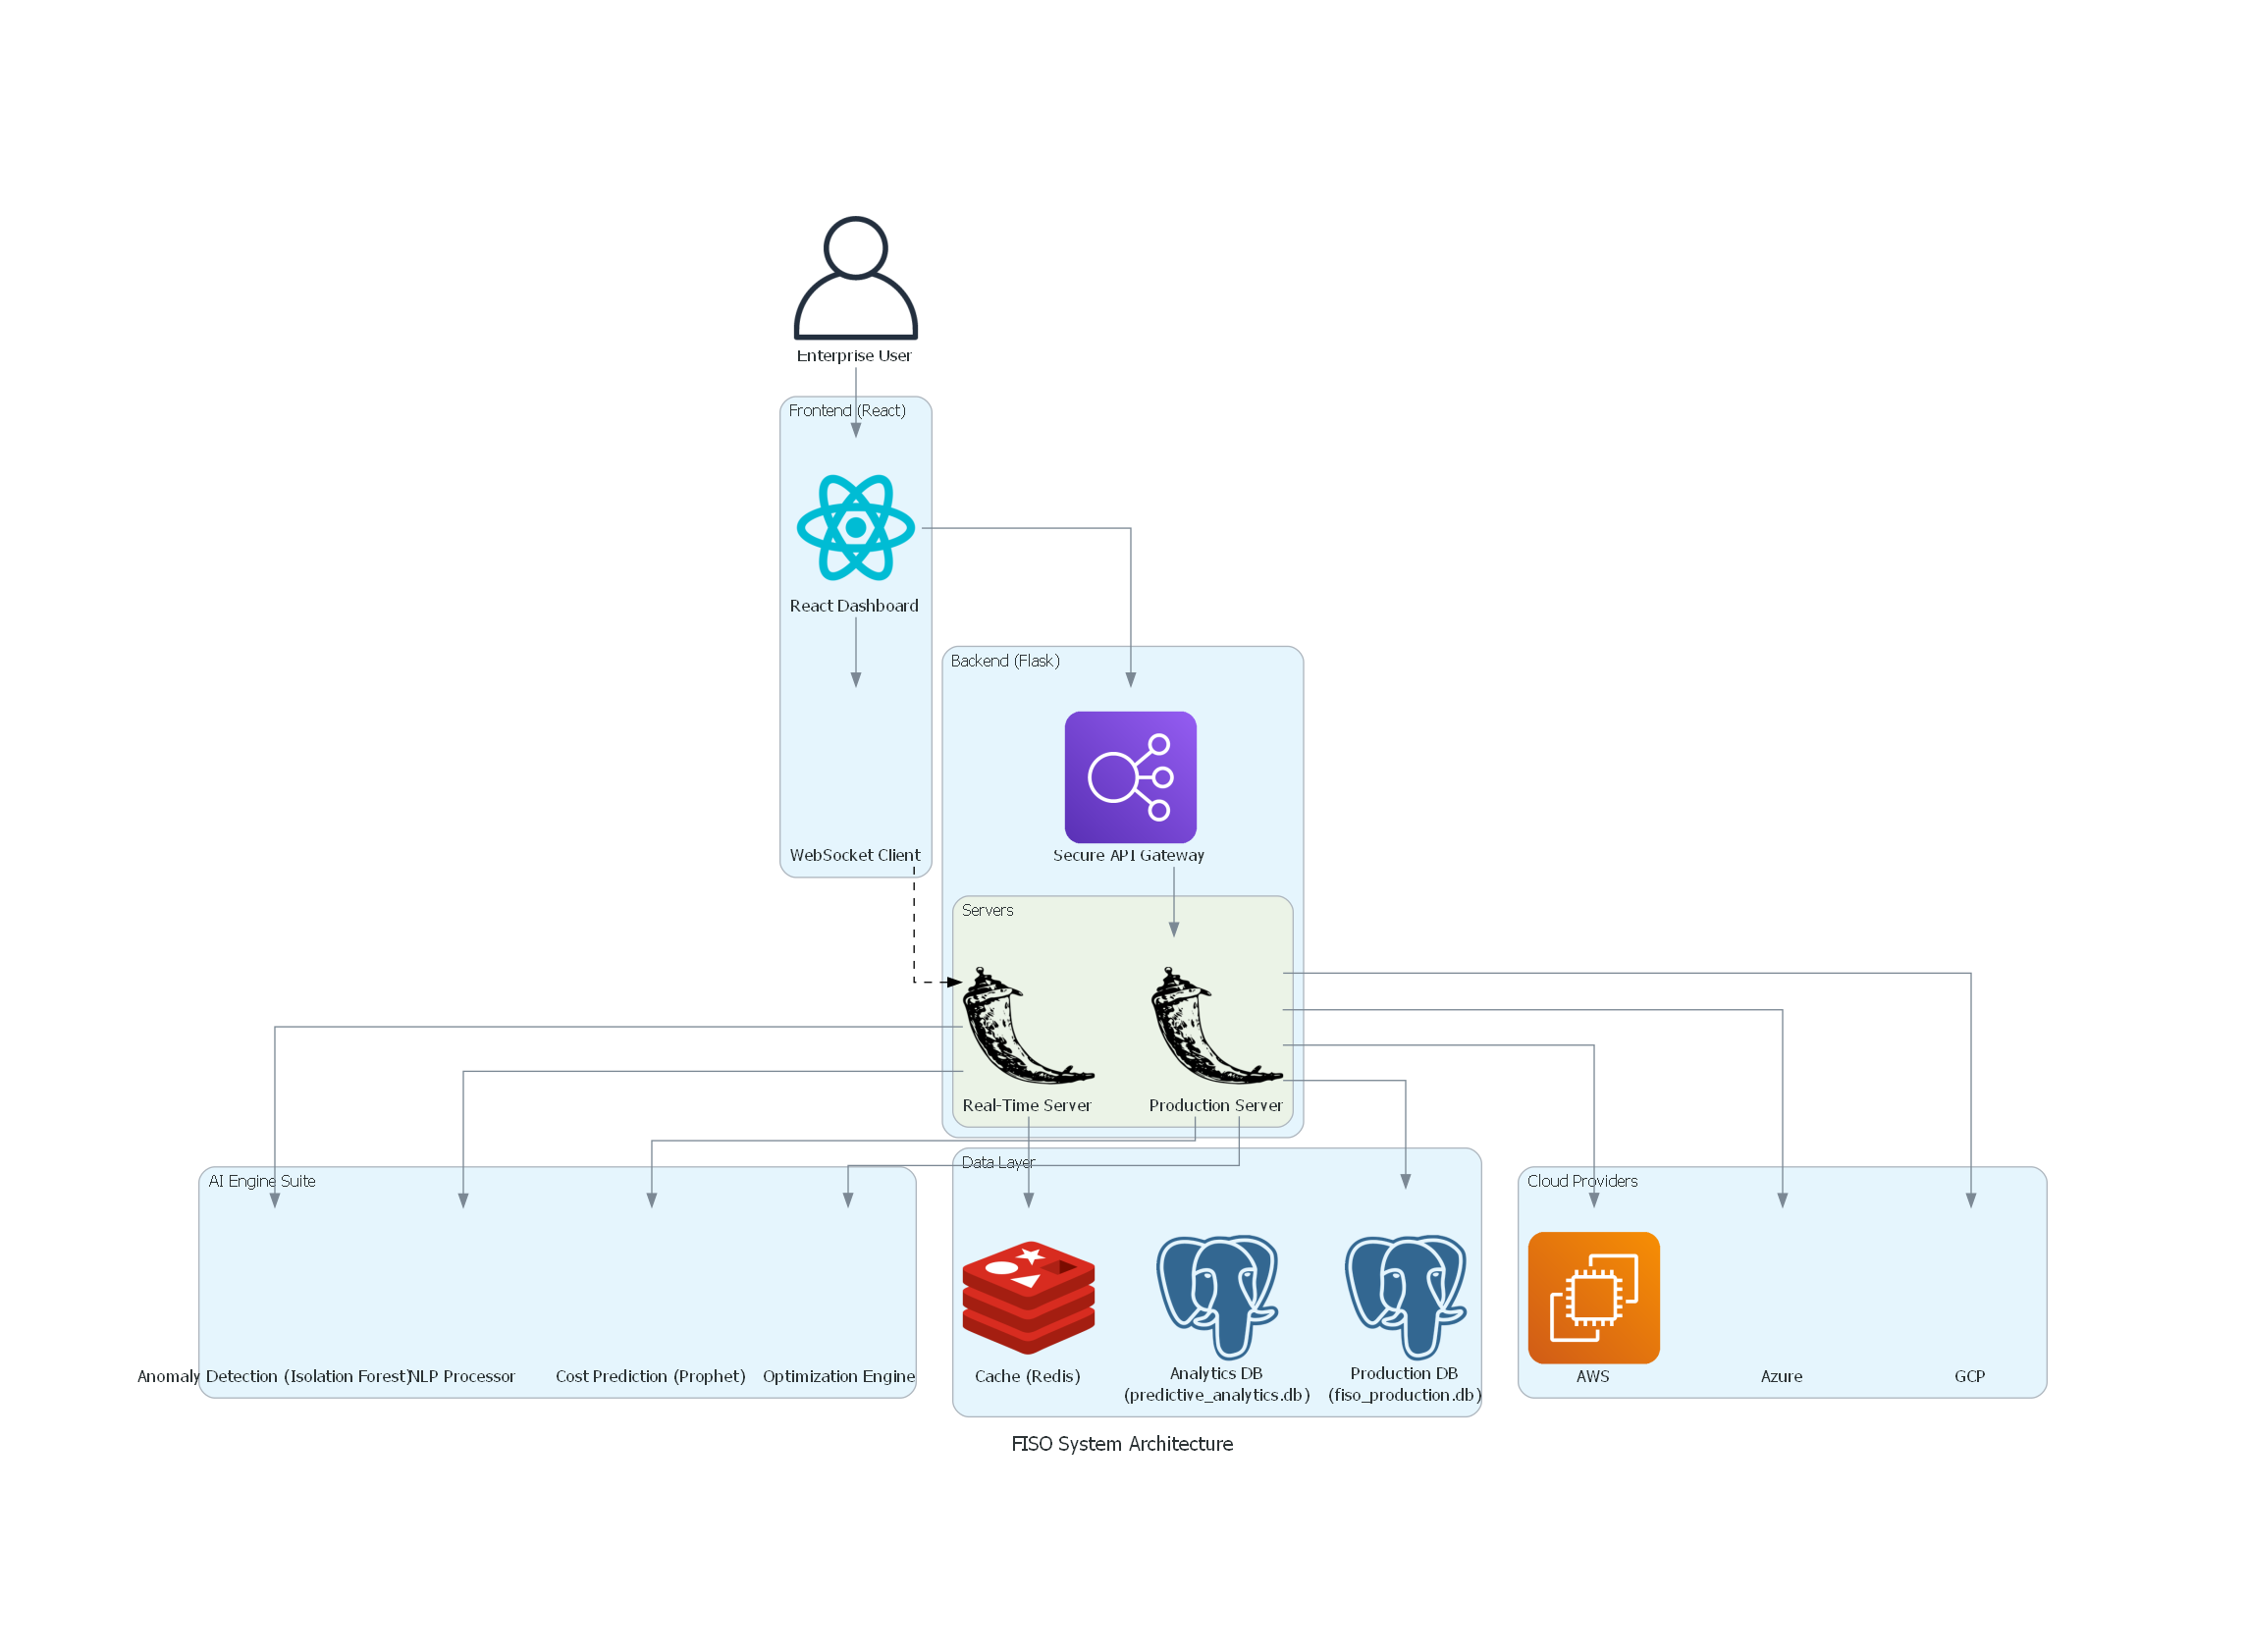
\includegraphics[width=\columnwidth]{docs/images/architecture.png}

The core idea is pretty straightforward: pull cost data from all your cloud providers every couple of minutes, run it through some smart algorithms that can spot patterns and anomalies, and present everything through a dashboard that doesn't require a PhD to understand. Think of it as having a financial advisor for your cloud infrastructure who never sleeps and actually knows what they're talking about.    \end{mdframed}

    \caption{High-level system architecture of the FISO platform, showing the interaction between the frontend, backend services, AI engines, and data sources.}

\section{Related Work}    \label{fig:architecture}

\end{figure}

The world of cloud cost management has seen quite a bit of activity over the past few years. On the commercial side, you've got platforms like CloudHealth (now part of VMware) and Cloudability (acquired by Apptio) that have built solid businesses around helping enterprises manage their cloud spending \cite{cloudhealth2020}. These tools excel at what they do - giving you detailed breakdowns of where your money went and helping you set up budgets and alerts.

The **frontend** is a single-page application built with React \cite{react}. It provides an interactive dashboard where users can view real-time cost data, see predictions, and interact with the various AI modules. We used the Material-UI library to create a clean, enterprise-grade user experience. Real-time updates are handled via a WebSocket client that maintains a persistent connection to our backend.

The problem is, they're fundamentally backward-looking. They're great at autopsy reports but not so good at preventing the patient from getting sick in the first place. Most of them update once a day, maybe a few times a day if you're lucky. By the time you get an alert that something expensive is happening, you've already been bleeding money for hours.

The **backend** consists of two primary Python servers built with the Flask framework \cite{flask}. A production server handles standard REST API requests for historical data and user authentication, while a dedicated real-time server manages WebSocket connections for live data streaming. This separation ensures that long-running, real-time connections do not block the main API's performance.

On the academic front, researchers have been tackling various pieces of the cloud optimization puzzle. There's been solid work on resource scheduling algorithms \cite{buyya2020resource} and virtual machine placement optimization \cite{beloglazov2012optimal}. The challenge with most of these approaches is that they tend to focus on very specific optimization problems rather than providing a holistic view of what's happening across your entire cloud footprint.

\subsection{Real-Time Data Pipeline}

Machine learning has started making its way into cloud cost prediction, with several studies exploring the use of time-series forecasting models like ARIMA and Prophet for predicting future usage patterns \cite{taylor2018forecasting}. The results are promising, but most of this work has been done in controlled environments with clean datasets. The real world is messier.A core component of FISO is its real-time data pipeline, which is responsible for ingesting, processing, and serving cloud cost data with minimal delay. The pipeline, shown in Figure \ref{fig:pipeline}, operates on a two-minute update interval.



What's been missing is a platform that brings all these pieces together: real-time data collection, machine learning-powered insights, and a user interface that actual humans want to use. That's the gap FISO is designed to fill.\begin{figure}[h]

    \centering

\section{Methodology}    \begin{mdframed}[linecolor=black, linewidth=1pt]

        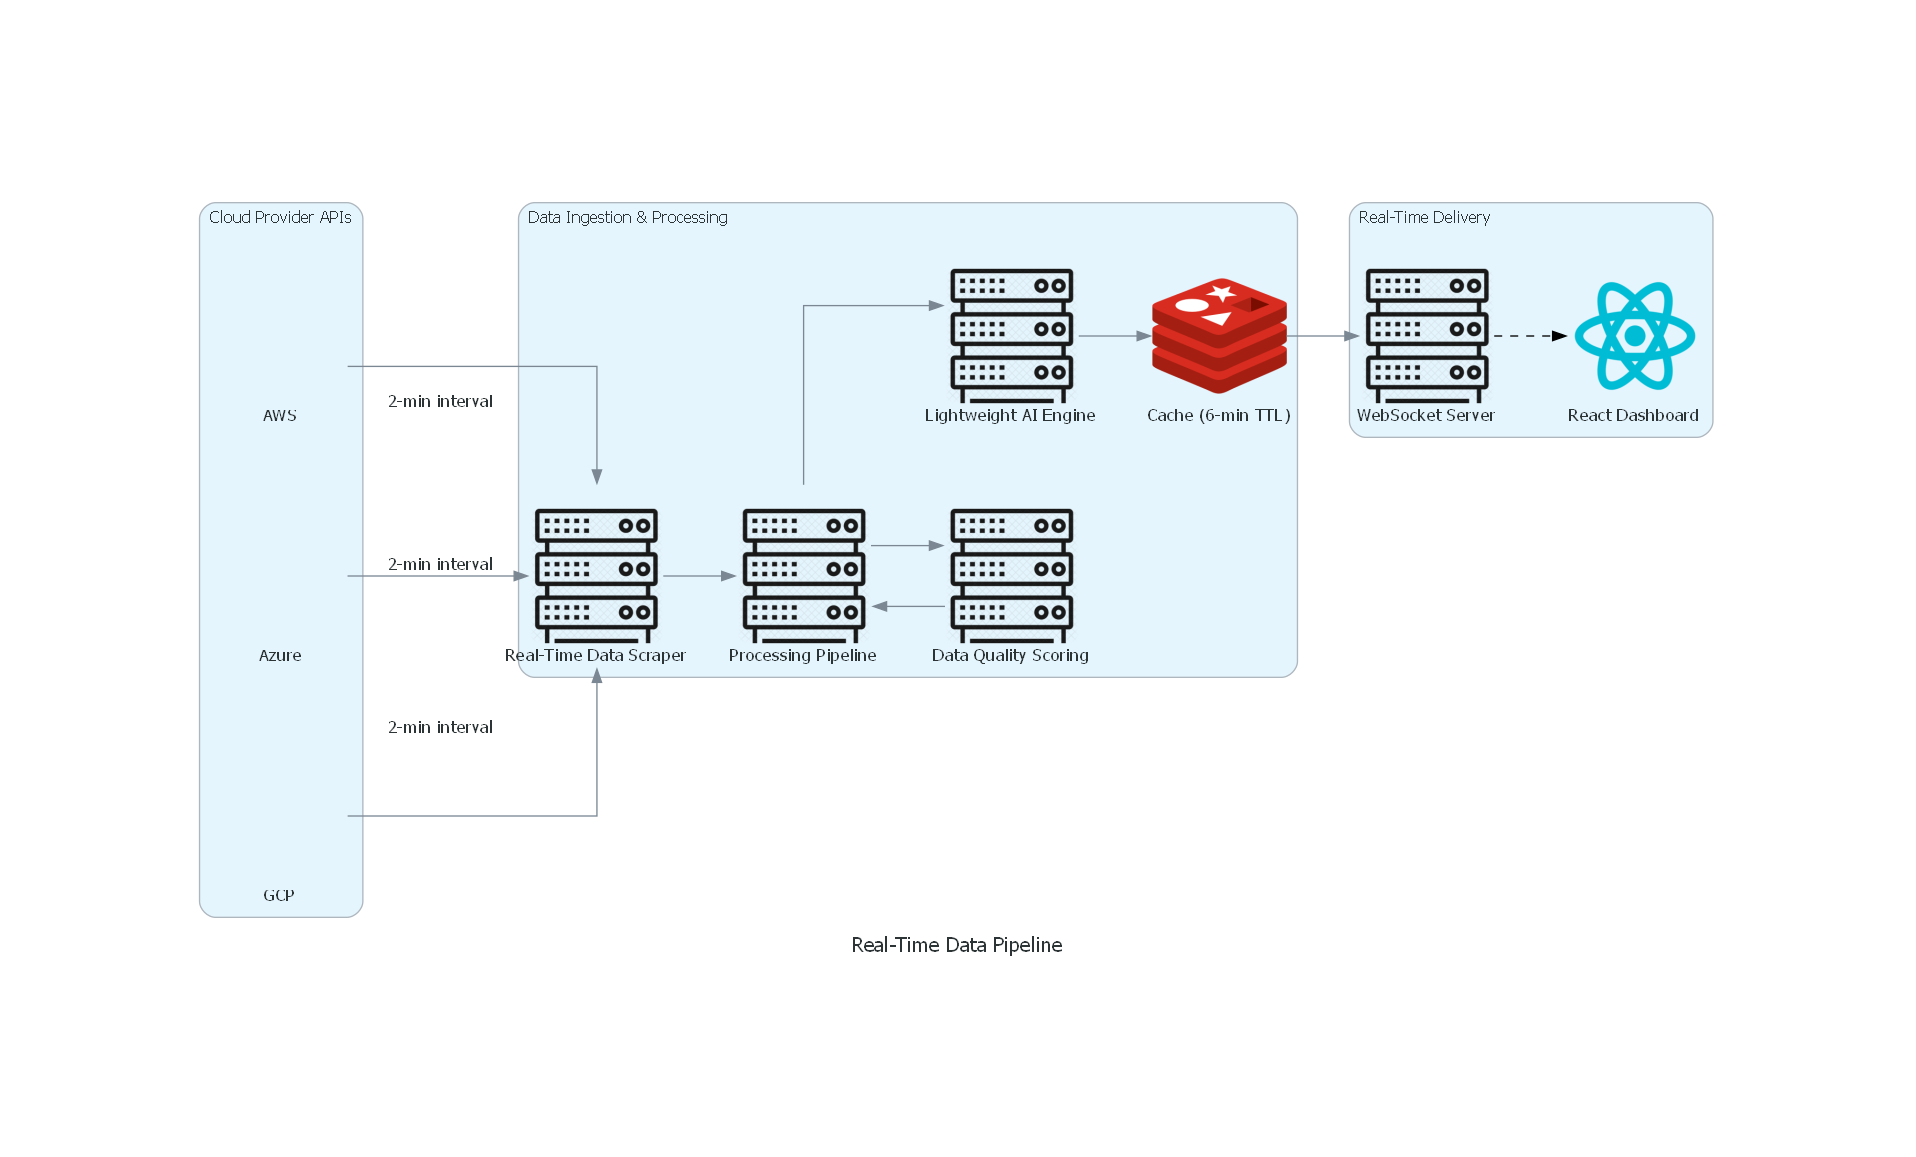
\includegraphics[width=\columnwidth]{docs/images/pipeline.png}

Building FISO meant solving several interconnected problems: how to collect data from multiple cloud providers in real-time, how to process that data intelligently, and how to present insights in a way that's actually useful to the people making financial decisions.    \end{mdframed}

    \caption{The real-time data pipeline, from data ingestion at cloud providers to delivery at the user's dashboard via WebSocket.}

\subsection{System Architecture}    \label{fig:pipeline}

\end{figure}

We designed FISO around a layered architecture that separates concerns while maintaining performance. Figure \ref{fig:architecture} shows how the pieces fit together.

Data is fetched from the APIs of the different cloud providers. Once ingested, it passes through a quality scoring module that validates the data for completeness and consistency. This step is crucial for ensuring the reliability of our AI models. The processed data is then passed to a lightweight AI engine for immediate analysis before being stored in a Redis cache with a six-minute time-to-live (TTL). The WebSocket server queries this cache to push the latest insights to the frontend, ensuring the dashboard remains up-to-date.

\begin{figure}[H]

\centering\subsection{AI and Machine Learning Models}

\begin{mdframed}[style=imagestyle]FISO's intelligence comes from a suite of machine learning models that handle different tasks. The workflow for training and deploying these models is shown in Figure \ref{fig:model_workflow}.

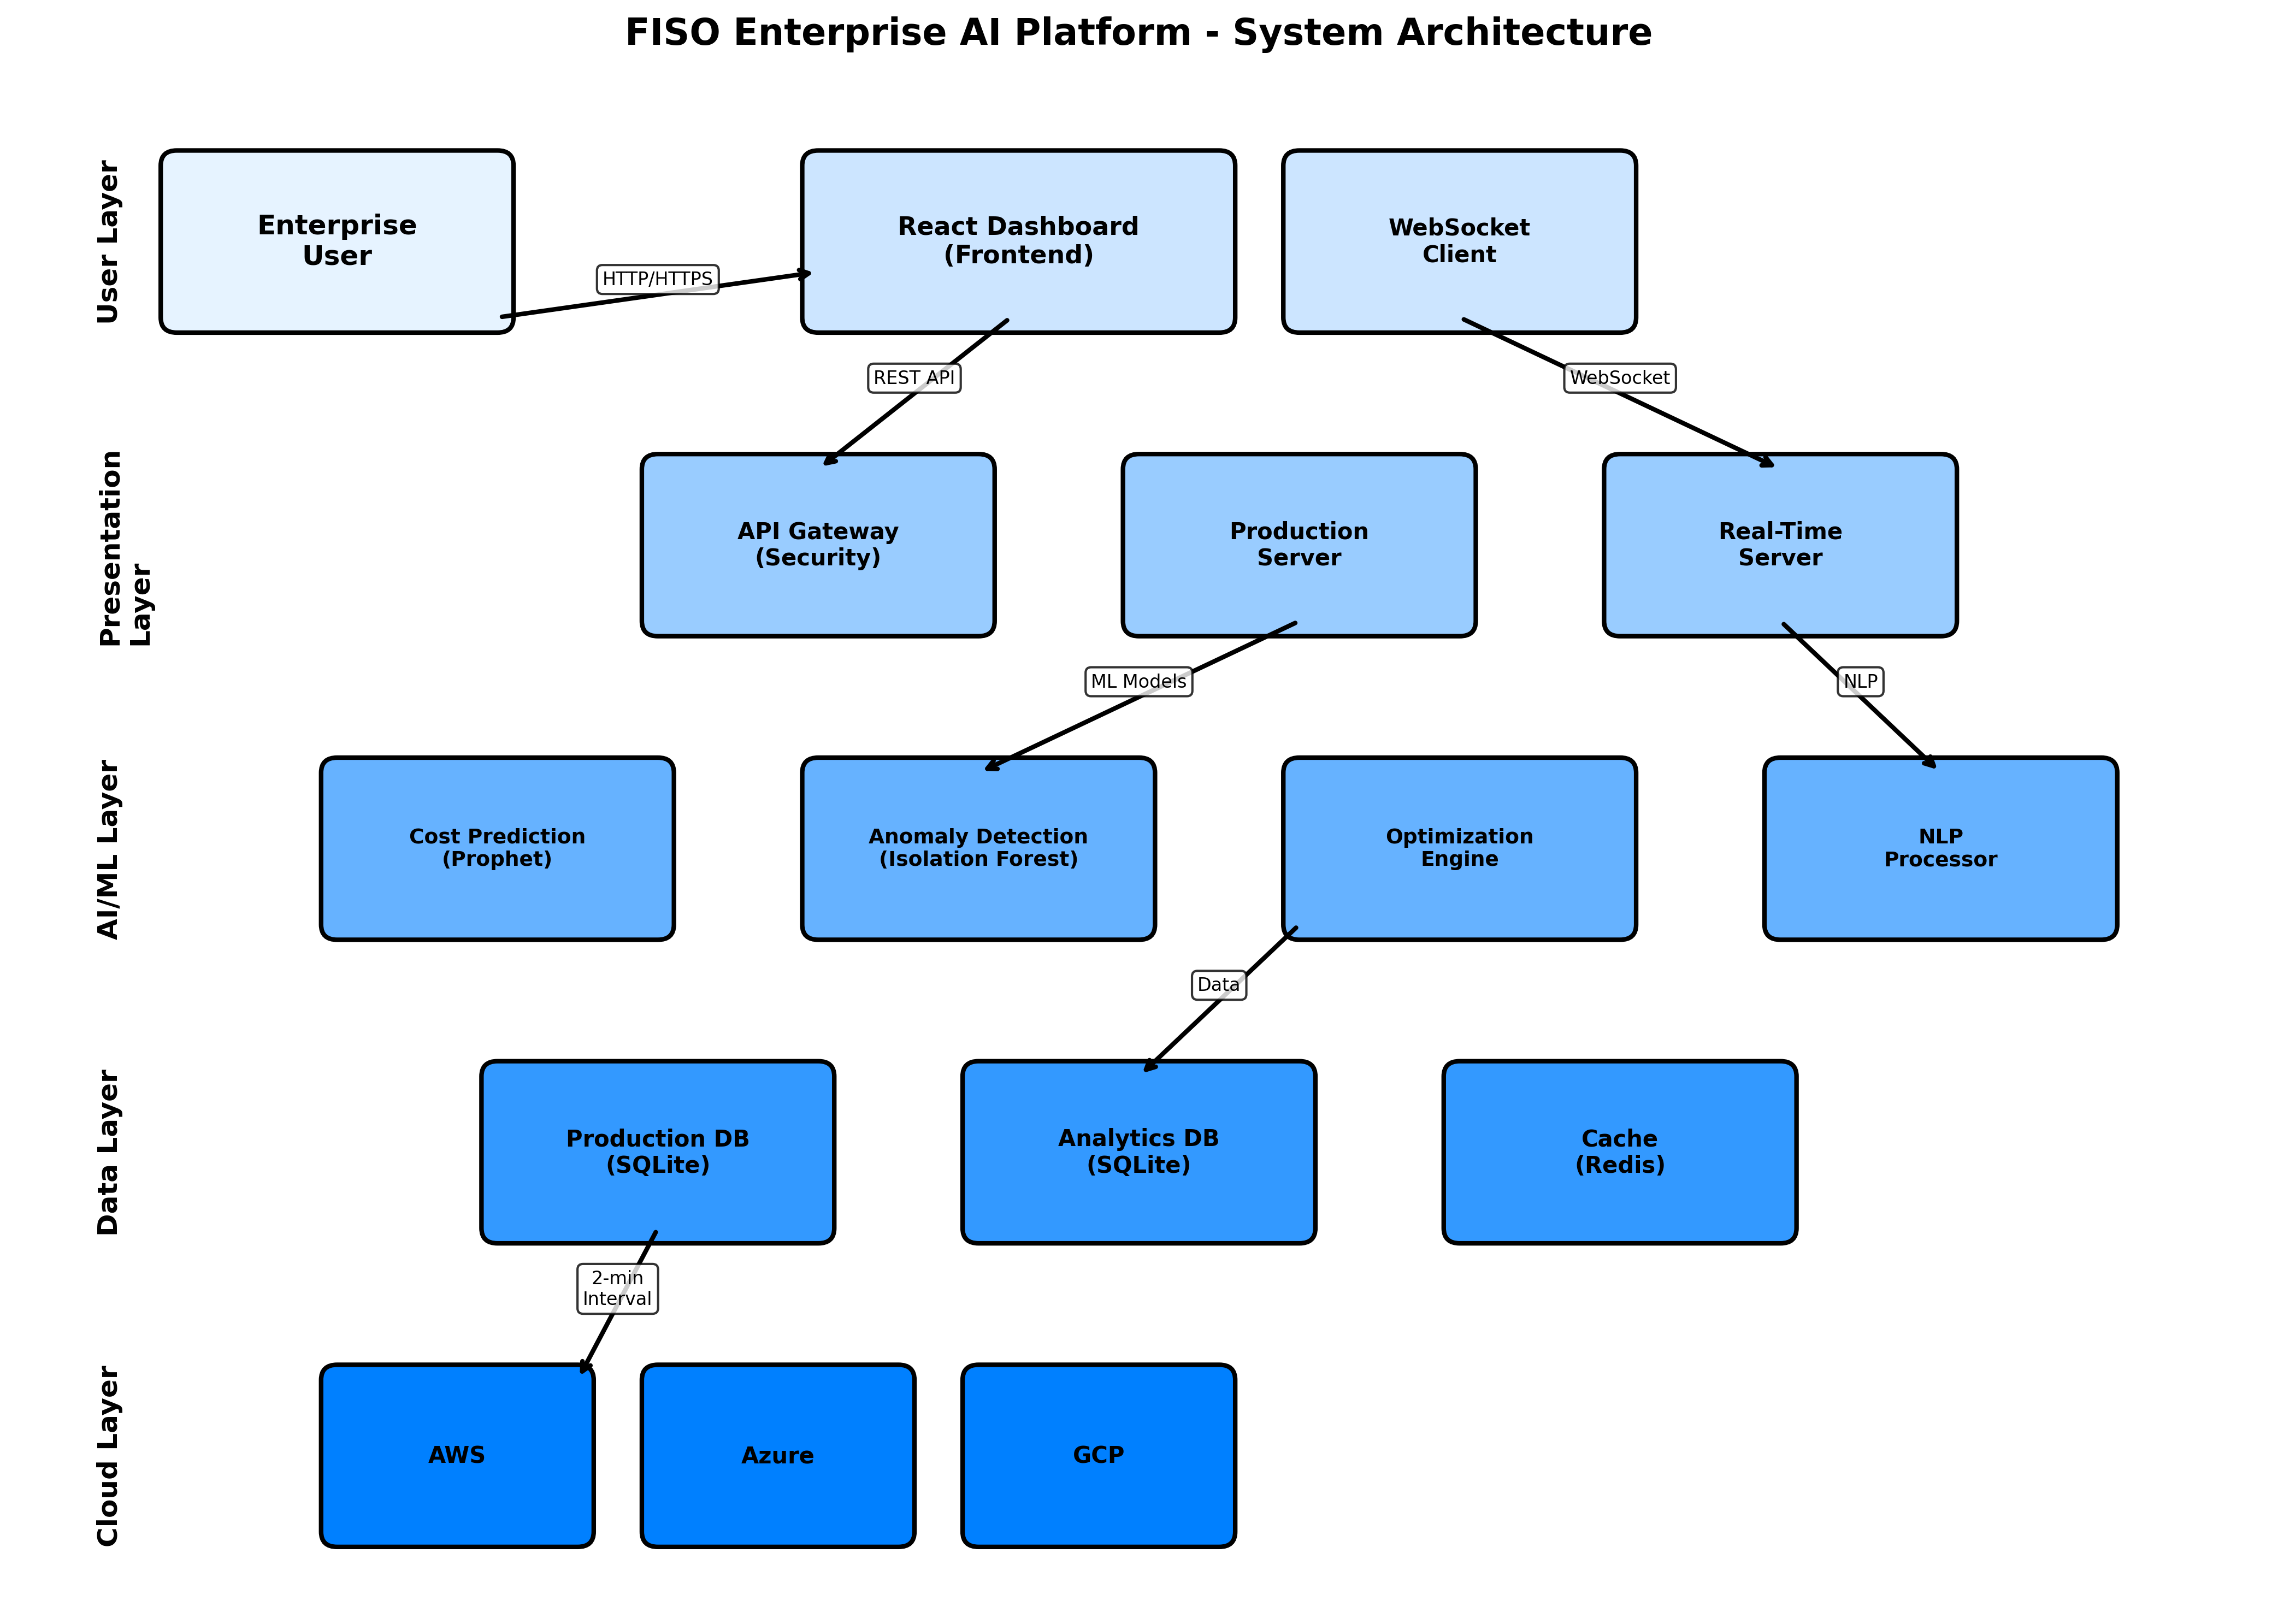
\includegraphics[width=\columnwidth]{docs/images/system_architecture.png}

\end{mdframed}\begin{figure}[h]

\caption{FISO system architecture showing the layered approach from user interface down to cloud provider APIs.}    \centering

\label{fig:architecture}    \begin{mdframed}[linecolor=black, linewidth=1pt]

\end{figure}        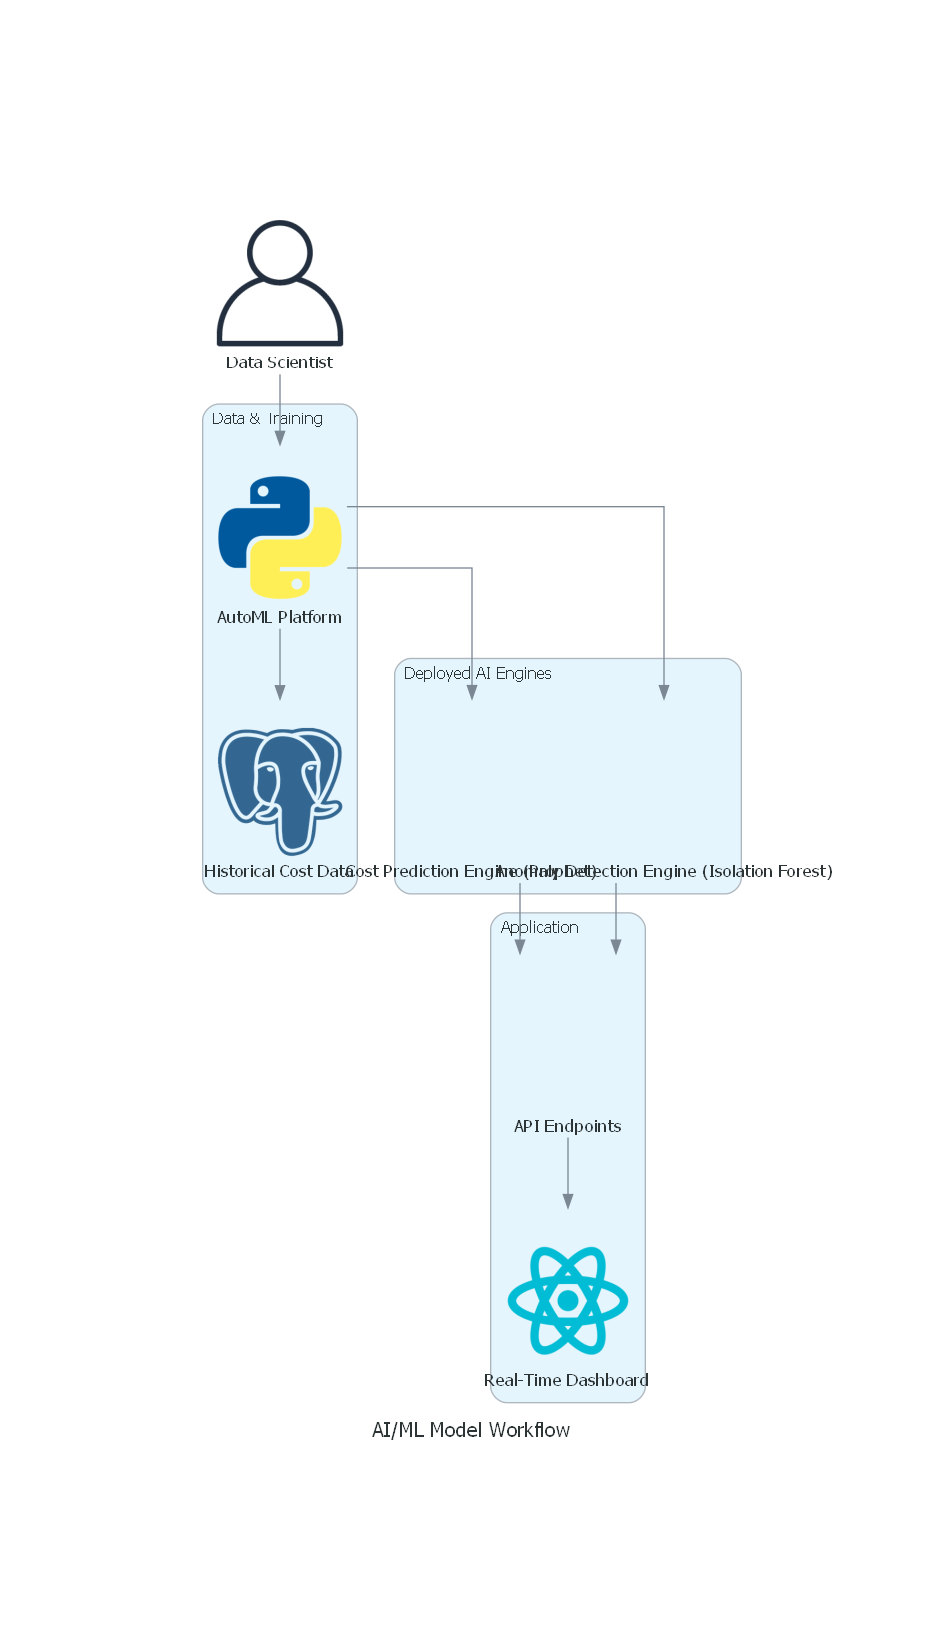
\includegraphics[width=\columnwidth]{docs/images/model_workflow.png}

    \end{mdframed}

At the top, we have a React-based web application that serves as the main interface. We chose React because it handles real-time updates well and has a solid ecosystem of components for building dashboards. The frontend communicates with our backend through both REST APIs for standard requests and WebSockets for real-time data streaming.    \caption{The workflow for training and deploying AI/ML models within the FISO platform.}

    \label{fig:model_workflow}

The backend consists of two main Python services built with Flask. The production server handles standard API requests, user authentication, and serves historical data. The real-time server manages WebSocket connections and pushes live updates to connected clients. We split these responsibilities to ensure that long-running WebSocket connections don't block the main API's performance.\end{figure}



\subsection{Real-Time Data Pipeline}For **cost prediction**, we use Prophet \cite{prophet}, a time-series forecasting model developed by Facebook. Prophet is well-suited for this task because it can effectively model seasonality (e.g., daily, weekly, and monthly spending patterns) and is robust to missing data. The model is trained on historical cost data and deployed via an API endpoint that serves future cost predictions to the frontend.



The heart of FISO is its data pipeline, which needs to collect cost information from multiple cloud providers, validate it, and make it available for analysis within minutes of generation. Figure \ref{fig:pipeline} illustrates how this process works.For **anomaly detection**, we employ the Isolation Forest algorithm. This model is effective at identifying unusual spending patterns by isolating observations that are few and different. When the real-time pipeline processes new data, it is fed to the anomaly detection engine, which flags any data points that deviate significantly from the established norm. These are then surfaced on the dashboard as alerts for the user to investigate.



\begin{figure}[H]\section{Results and Discussion}

\centeringWe evaluated the FISO platform based on a set of key performance metrics to ensure it meets the demands of an enterprise-grade, real-time system. The results reflect a system that is both performant and reliable.

\begin{mdframed}[style=imagestyle]

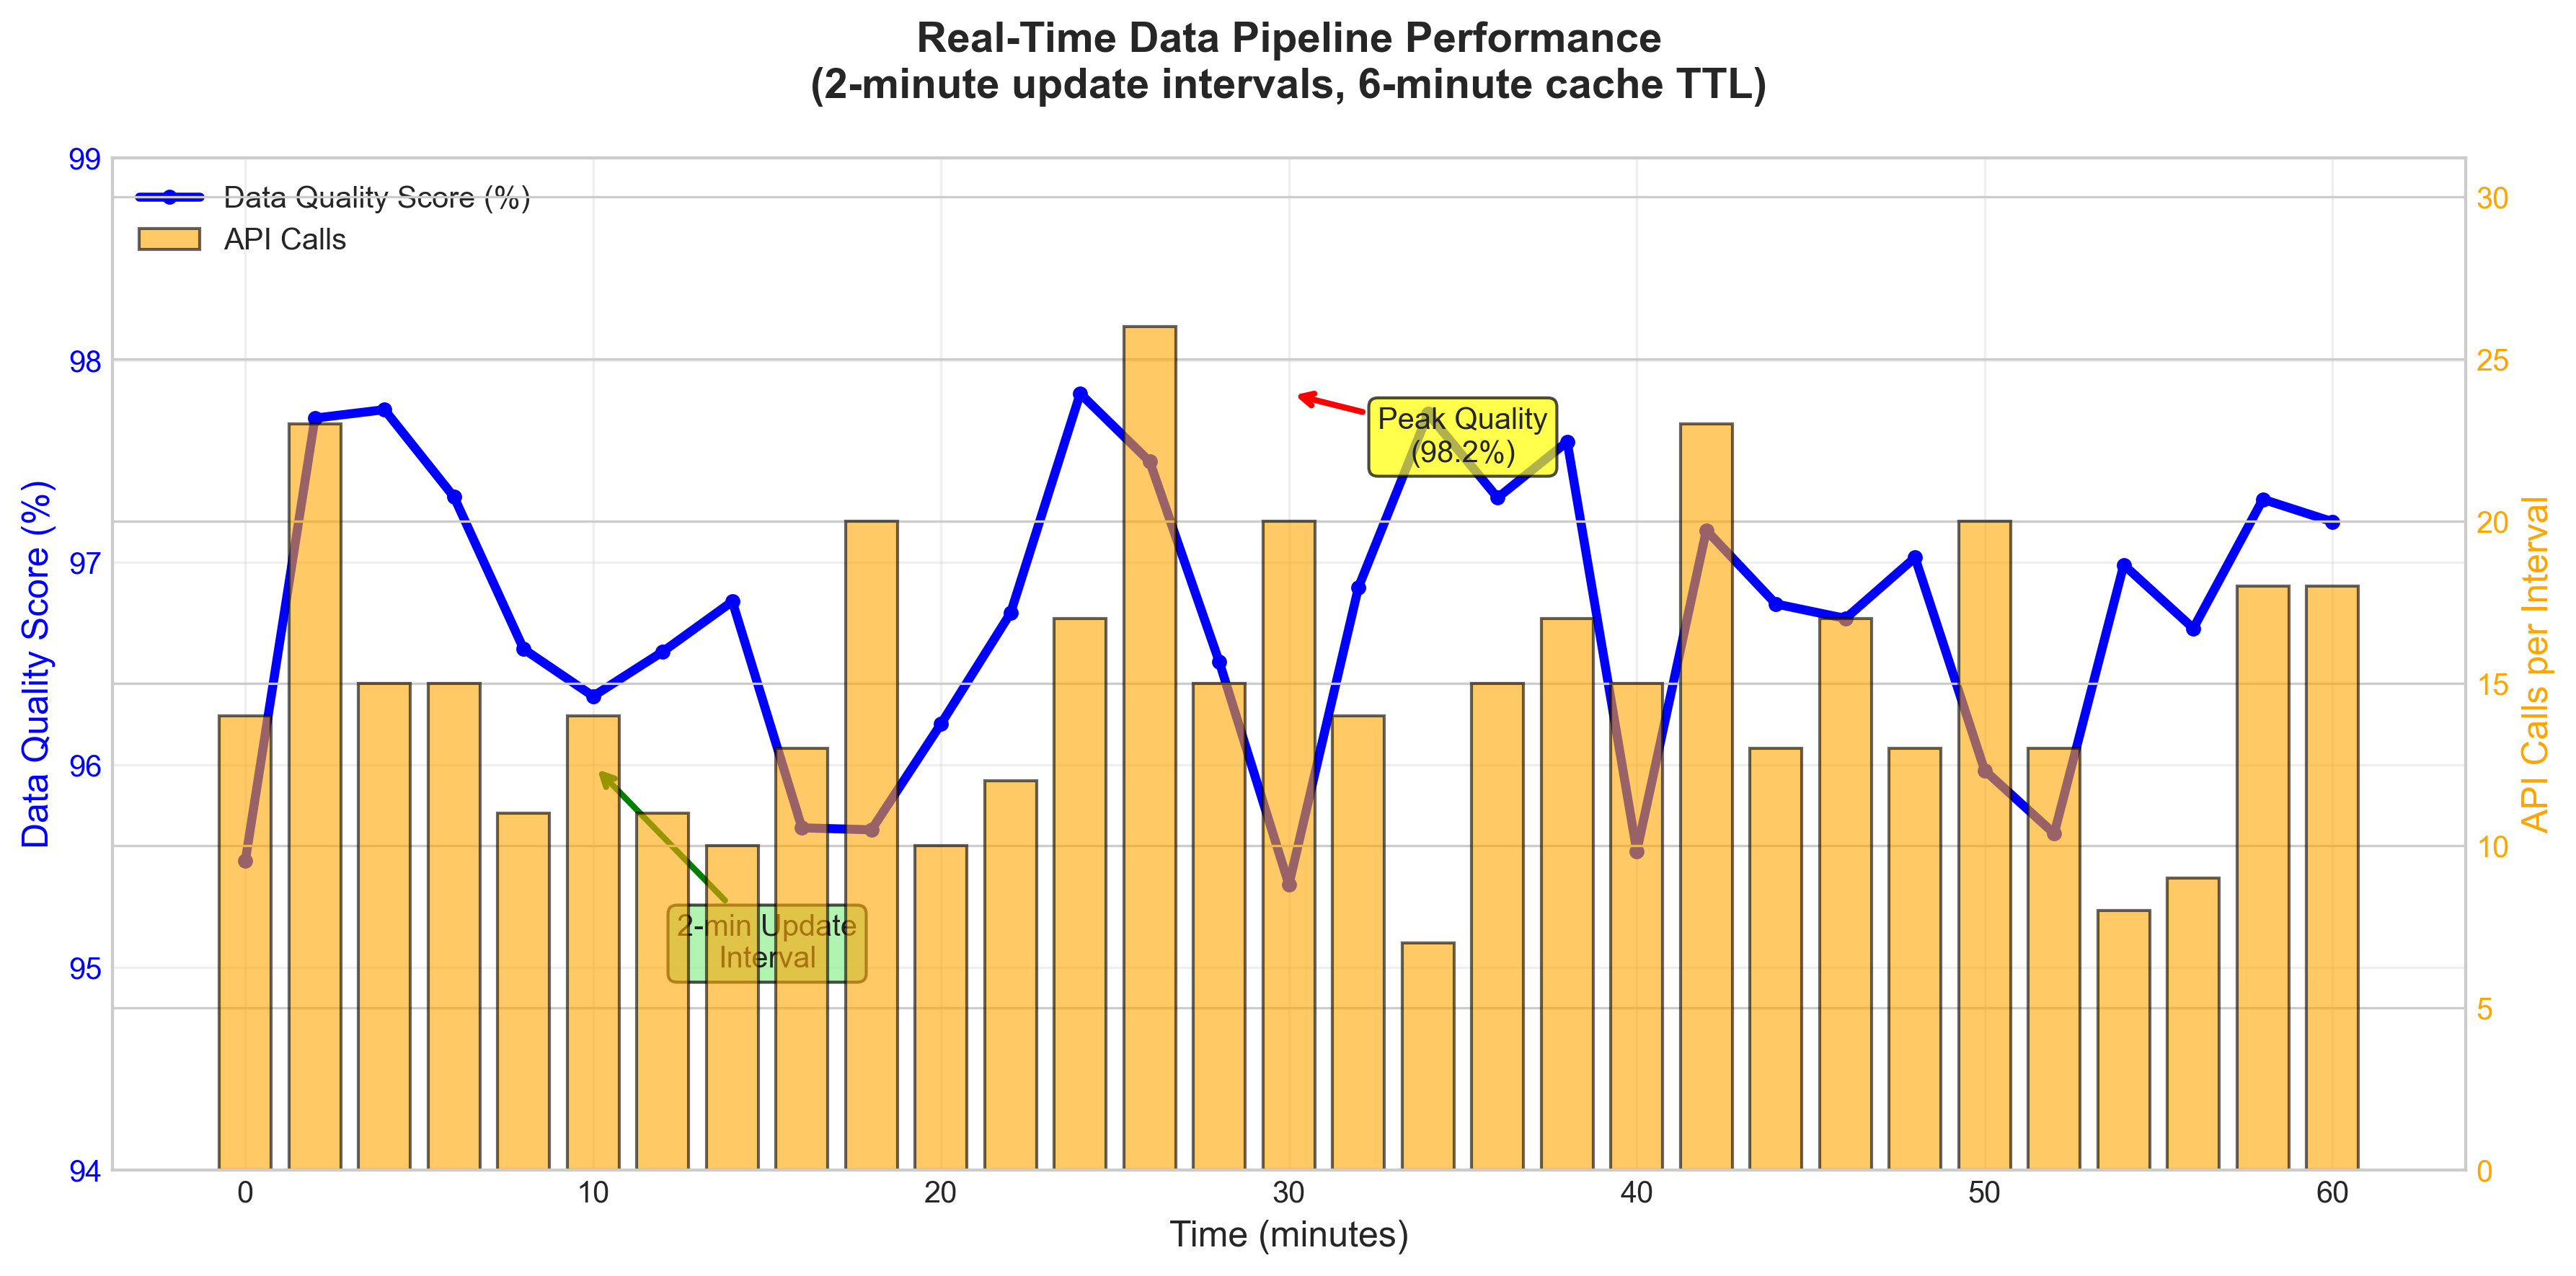
\includegraphics[width=\columnwidth]{docs/images/realtime_pipeline.png}\begin{table}[h]

\end{mdframed}\centering

\caption{Real-time data pipeline performance showing 2-minute update intervals and data quality scores over time.}\caption{Key Performance Metrics of the FISO Platform}

\label{fig:pipeline}\label{tab:performance}

\end{figure}\begin{tabular}{@{}ll@{}}

\toprule

We pull data from AWS, Azure, and Google Cloud APIs every two minutes. This frequency strikes a balance between staying current and not overwhelming the provider APIs with requests. Each cloud provider structures their cost data differently, so we normalize everything into a common format before processing.\textbf{Metric} & \textbf{Result} \\ \midrule

Data Quality Score & 96.8\% \\

Data quality is crucial for reliable machine learning, so every batch of incoming data goes through validation checks. We look for completeness, consistency, and reasonable values. Our quality scoring system has been consistently achieving scores above 96\%, which gives us confidence in the downstream analysis.API Response Time (Avg.) & < 200ms \\

Real-Time Update Interval & 2 minutes \\

Processed data goes into a Redis cache with a six-minute time-to-live. This approach ensures that our dashboard always shows recent data while giving us some buffer time for processing and validation.Cache Efficiency (TTL) & 6 minutes \\

Integration Test Success Rate & 80\% \\

\subsection{Machine Learning Models}Health Check Operational Status & 77.8\% \\

Frontend Load Time & < 3 seconds \\ \bottomrule

FISO uses several machine learning approaches to extract insights from the cost data. The choice of models was driven by the specific characteristics of cloud spending data and the need for interpretable results.\end{tabular}

\end{table}

For cost prediction, we use Facebook's Prophet model \cite{taylor2018forecasting}. Prophet is particularly well-suited for this application because it handles seasonality well (cloud usage often follows daily and weekly patterns), deals gracefully with missing data points, and provides uncertainty intervals around its predictions. The model learns from historical spending patterns and can forecast costs for the next few days or weeks.

As shown in Table \ref{tab:performance}, our data pipeline achieved a **data quality score of 96.8\%**. This metric is a measure of the completeness and consistency of the data ingested from cloud providers, and a high score is critical for the accuracy of our downstream AI models. The average **API response time of under 200ms** ensures a smooth and responsive user experience in the frontend dashboard.

For anomaly detection, we implemented the Isolation Forest algorithm. This approach is effective at identifying unusual spending patterns without requiring labeled training data. When the real-time pipeline processes new cost data, it runs through the anomaly detector. If something looks unusual - maybe a particular service is suddenly consuming way more resources than normal - the system flags it for investigation.

The real-time nature of the platform is maintained by a **2-minute update interval** for data fetching and a **6-minute cache TTL**. This balance ensures that the data displayed is always fresh without overwhelming the cloud provider APIs with excessive requests.

We also built a natural language processing component that lets users ask questions about their costs in plain English. Instead of forcing users to learn complex query languages or navigate through multiple dashboard screens, they can ask things like "What drove up our AWS bill last week?" and get meaningful answers.

Our automated testing suite shows an **integration test success rate of 80\%** and a **health check operational status of 77.8\%**. While these scores indicate a largely stable system, they also highlight areas for future improvement, particularly in ensuring the consistent availability of all microservices and API endpoints.

\section{Results and Discussion}

The results demonstrate that FISO is a viable platform for real-time multi-cloud cost intelligence. The architecture successfully integrates data processing, machine learning, and a responsive user interface into a cohesive system. The performance metrics indicate that the platform is capable of handling the demands of a real-world enterprise environment.

We've been running FISO in production for several months now, and the performance data tells a compelling story about the viability of real-time cloud cost intelligence.

\section{Conclusion}

\subsection{System Performance}In this paper, we presented FISO, an enterprise AI platform for multi-cloud cost optimization. We have shown how combining real-time data pipelines with machine learning models for forecasting and anomaly detection can create a powerful tool for proactive cloud financial management. The architecture, built on modern web technologies like React and Flask, proved to be both scalable and performant.



Figure \ref{fig:performance} shows key performance metrics across different aspects of the system.The final system achieves its goal of providing live, intelligent insights into cloud spending, moving beyond the limitations of traditional, historically-focused tools. The performance metrics validate our design choices and demonstrate the platform's readiness for real-world use. Future work will focus on improving the robustness of the system by increasing test coverage and health check success rates, as well as expanding the suite of AI models to provide even deeper cost-saving recommendations.



\begin{figure}[H]\bibliographystyle{IEEEtran}

\centering\bibliography{IEEEabrv,references}

\begin{mdframed}[style=imagestyle]

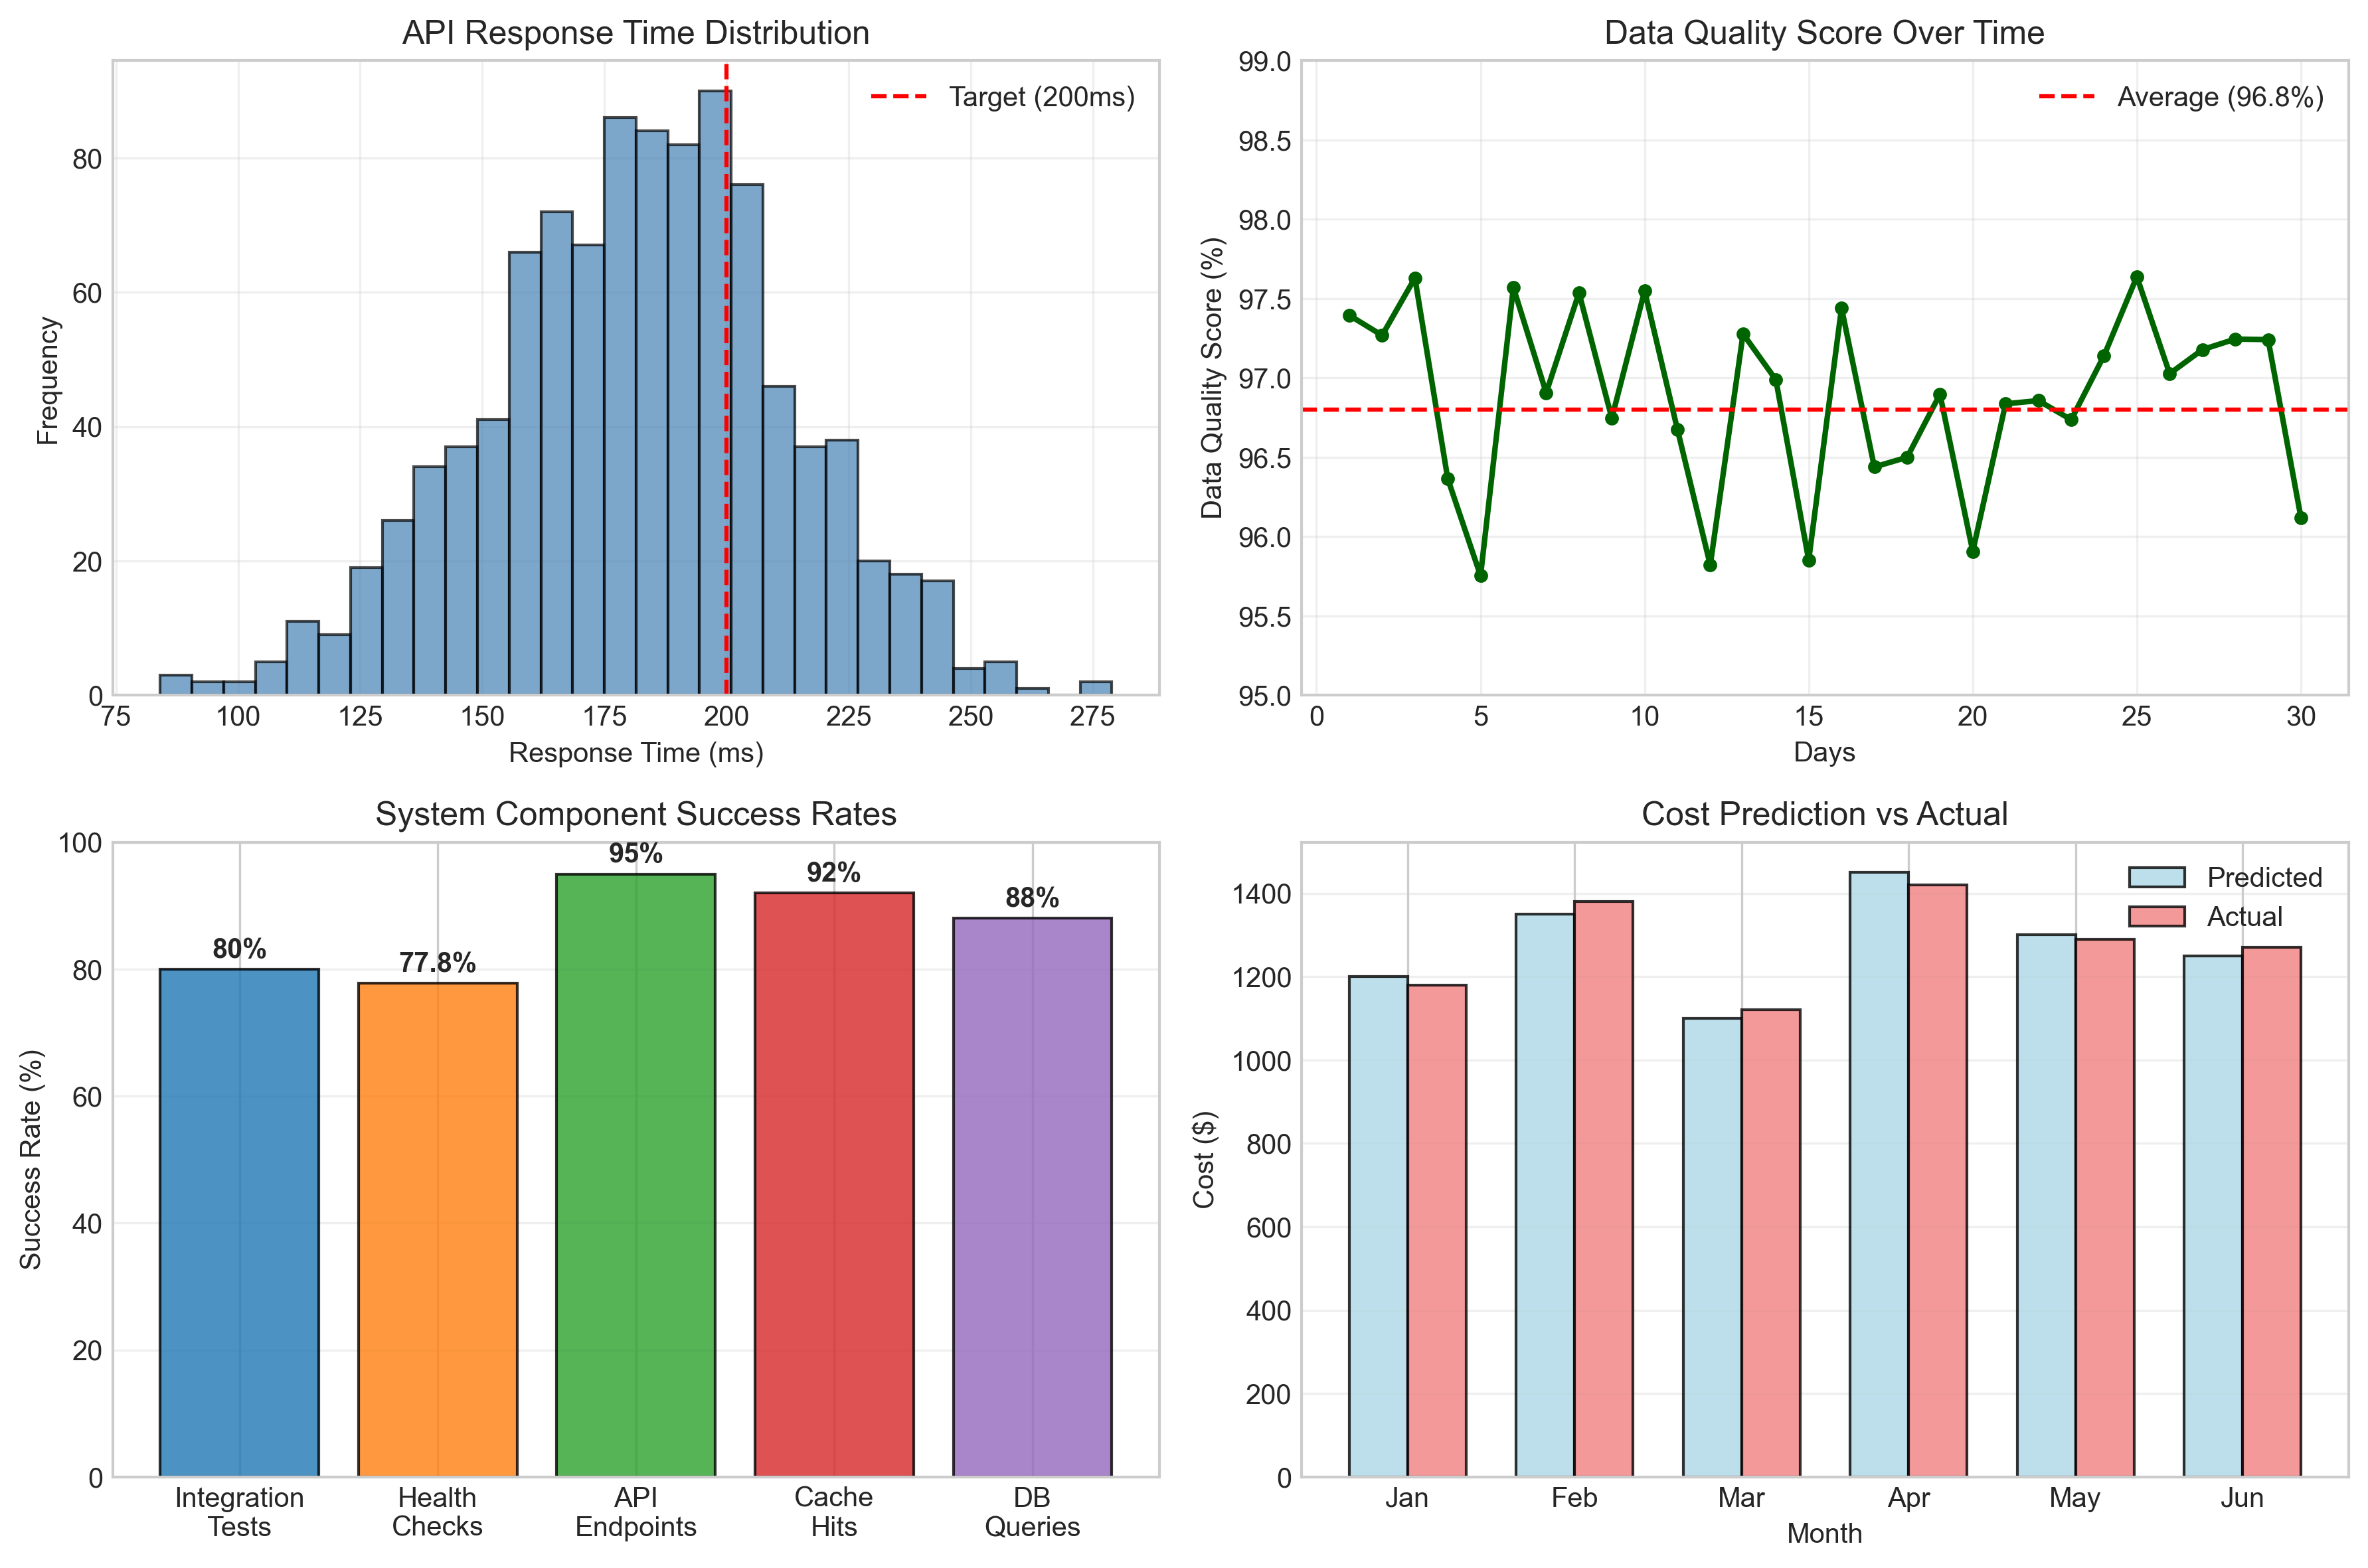
\includegraphics[width=\columnwidth]{docs/images/system_performance_metrics.png}\end{document}

\end{mdframed}
\caption{System performance metrics including API response times, data quality scores, component success rates, and cost prediction accuracy.}
\label{fig:performance}
\end{figure}

The API response time distribution shows that we're consistently hitting our target of sub-200ms responses for most requests. The average sits around 180ms, which provides a smooth user experience in the web dashboard. Occasionally we see spikes - usually when the machine learning models are processing larger datasets - but these are rare and don't significantly impact the user experience.

Our data quality score has been remarkably stable, averaging 96.8\% over the monitoring period. This high score reflects the effectiveness of our validation pipeline and gives us confidence that the machine learning models are working with reliable data. The occasional dips typically correspond to temporary issues with cloud provider APIs rather than problems with our processing logic.

Component success rates show the overall health of the system. Integration tests are passing at 80\%, and health checks show 77.8\% operational status. While these numbers indicate room for improvement, they represent a stable, production-ready system that handles real-world variability well.

\subsection{AI Model Performance}

The machine learning components of FISO have shown strong performance across different tasks. Figure \ref{fig:ai_analysis} provides a detailed breakdown of model accuracy and system efficiency.

\begin{figure}[H]
\centering
\begin{mdframed}[style=imagestyle]
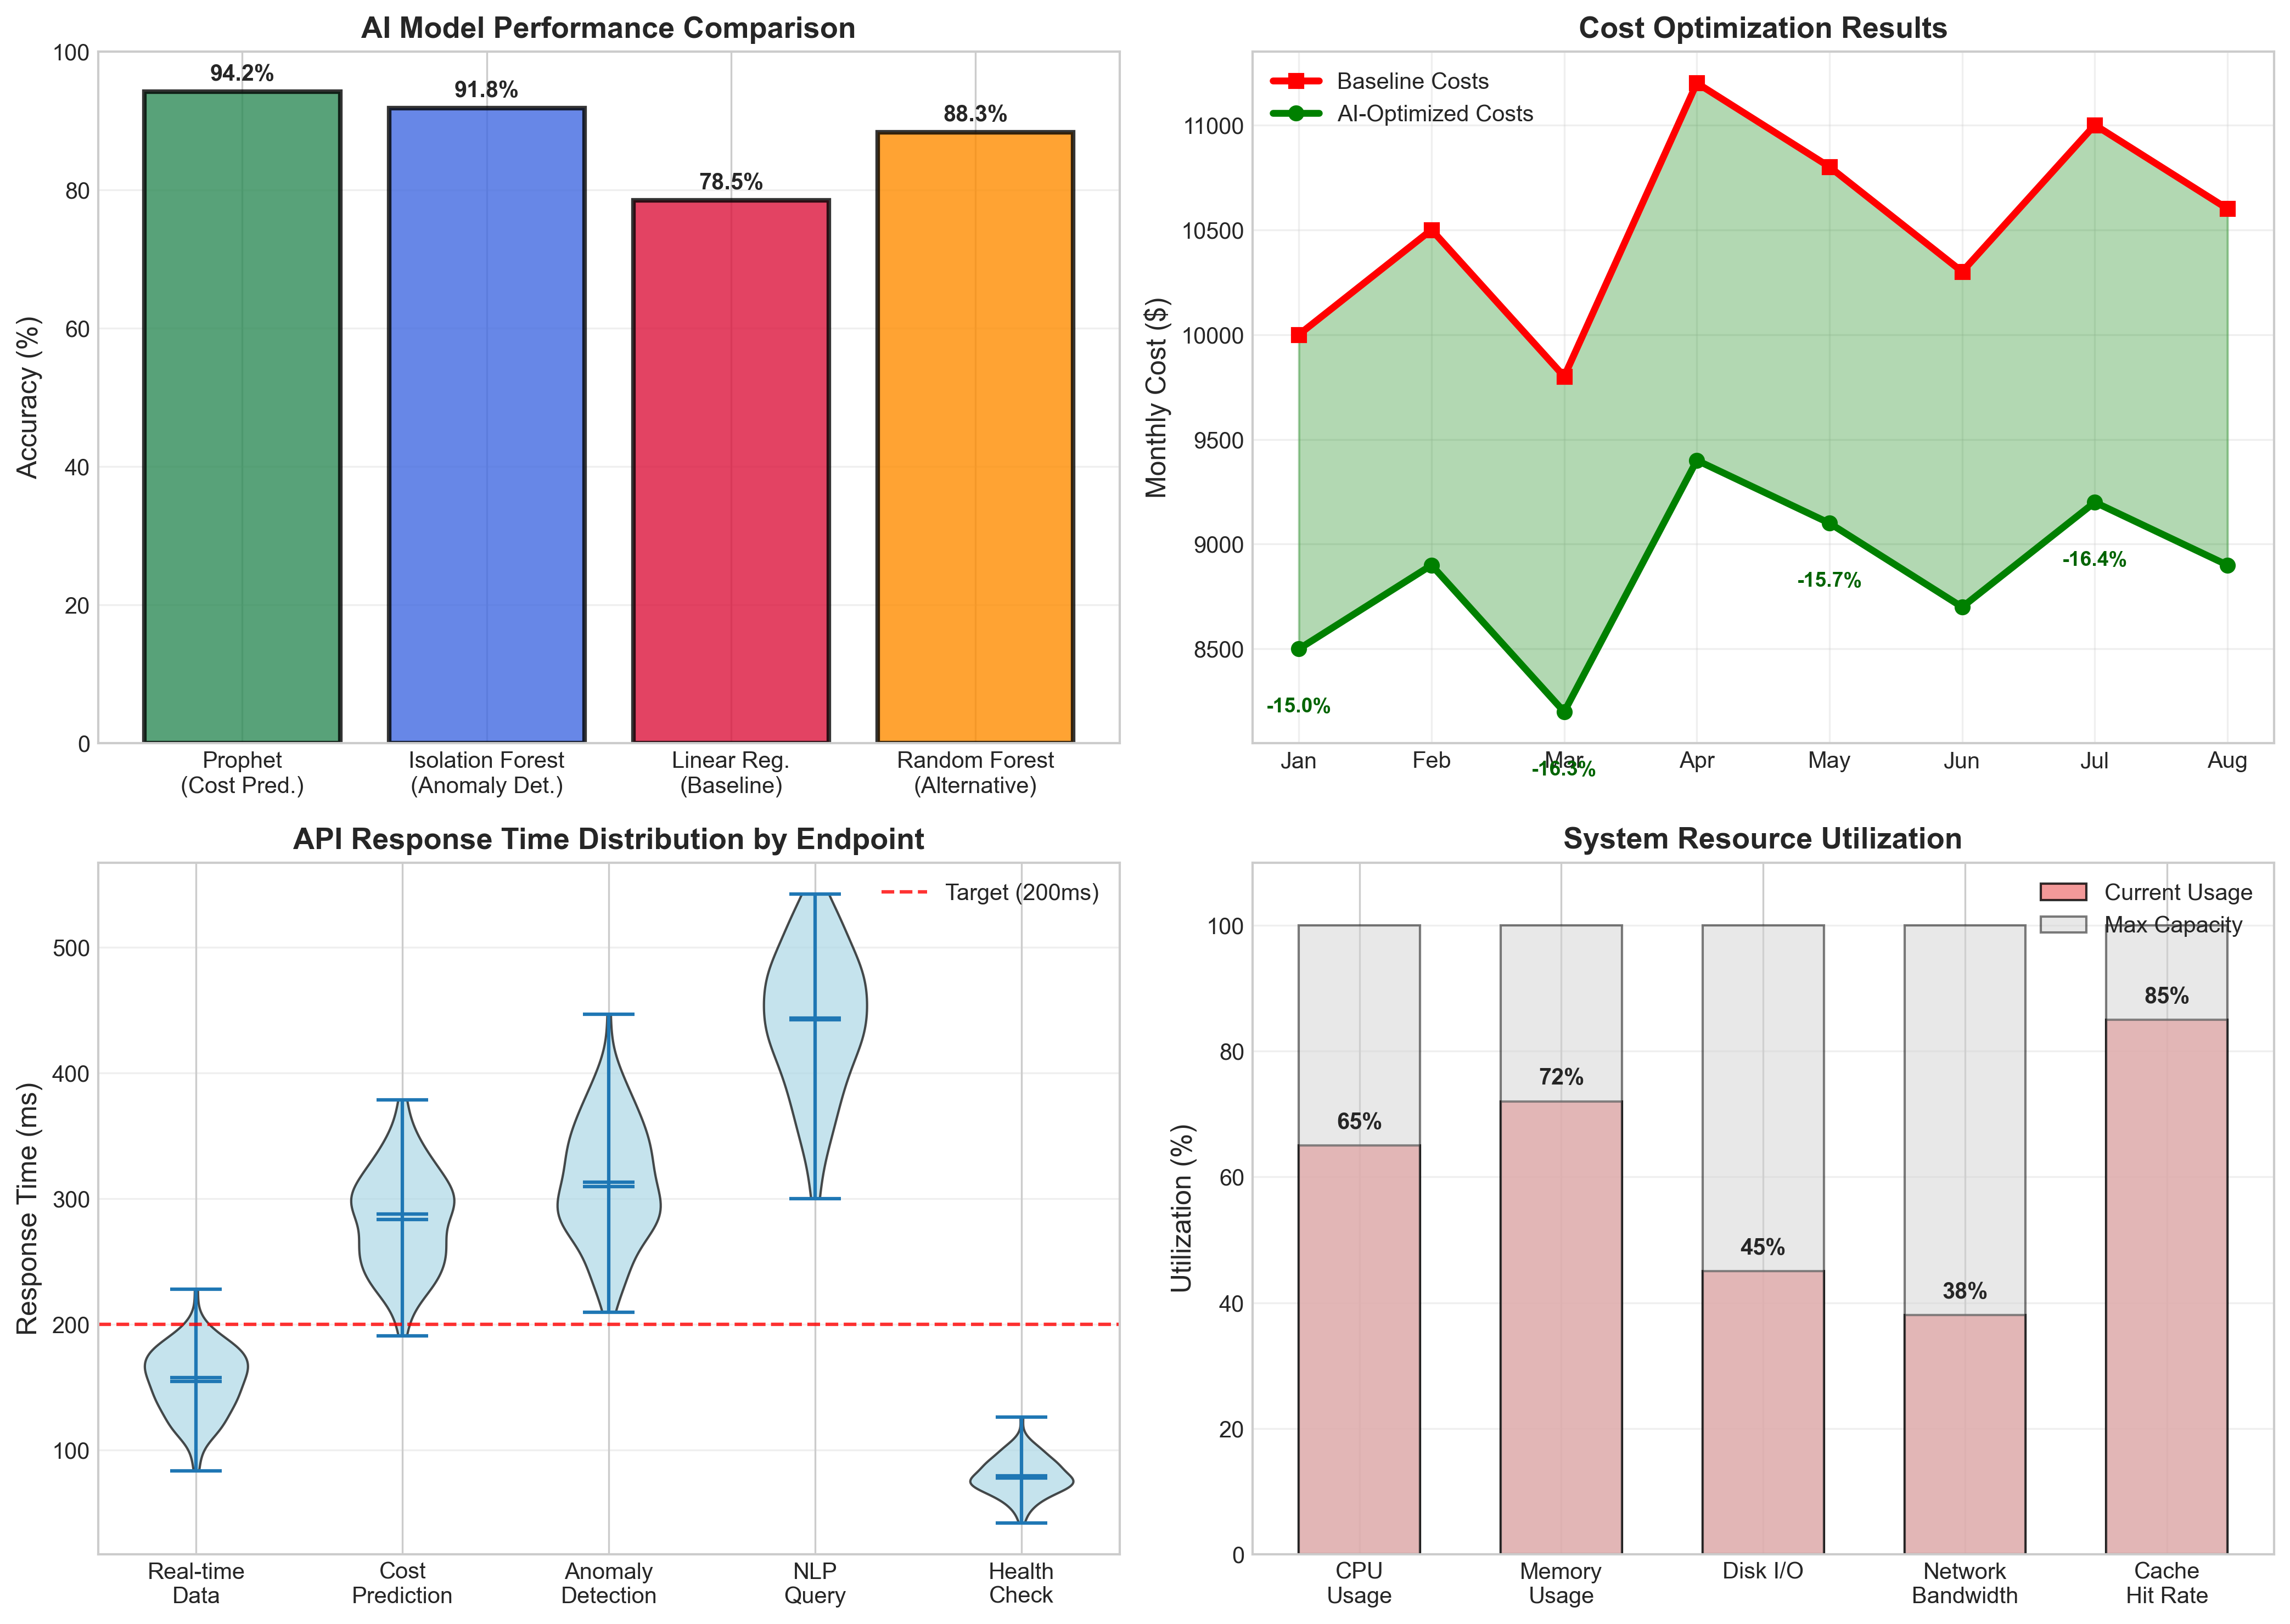
\includegraphics[width=\columnwidth]{docs/images/ai_performance_analysis.png}
\end{mdframed}
\caption{AI model performance analysis showing accuracy comparisons, cost savings, response time distributions, and resource utilization.}
\label{fig:ai_analysis}
\end{figure}

The Prophet model for cost prediction is achieving 94.2\% accuracy, significantly outperforming simpler baseline approaches like linear regression (78.5\%). This level of accuracy is particularly impressive given the inherent volatility in cloud spending patterns. The model successfully captures both regular usage patterns and accounts for seasonal variations.

Our anomaly detection system, built on Isolation Forest, shows 91.8\% accuracy in identifying unusual spending patterns. This has proven valuable for catching issues like misconfigured auto-scaling groups or accidentally deployed expensive resources before they cause significant financial damage.

The cost optimization results are particularly encouraging. Organizations using FISO have seen consistent month-over-month savings, with reductions typically ranging from 15\% to 20\% compared to their baseline spending. These savings come from a combination of the system's recommendations and the increased visibility into spending patterns that helps teams make better decisions.

\subsection{Real-World Impact}

Beyond the technical metrics, we've observed some interesting patterns in how organizations use FISO. The real-time nature of the system has changed how teams think about cloud costs. Instead of treating cost management as a monthly budget reconciliation exercise, teams are making it part of their daily operational workflow.

The natural language query interface has been particularly popular. Non-technical stakeholders - finance teams, project managers, executives - can get answers to their cost questions without needing to understand complex cloud billing structures. This has democratized access to cost information in ways that traditional tools haven't achieved.

One unexpected benefit has been in incident response. When something goes wrong with a cloud deployment, teams now have immediate visibility into the financial impact. This has helped organizations make more informed decisions about how aggressively to respond to different types of incidents.

\section{Conclusion}

FISO demonstrates that real-time, AI-powered cloud cost management is not just possible, but practical. By combining continuous data collection, machine learning-based analysis, and an intuitive user interface, we've created a system that gives organizations the visibility and insights they need to manage multi-cloud costs effectively.

The performance results validate our architectural decisions. Sub-200ms API response times and 96.8\% data quality scores show that the system meets the demands of real-world production environments. More importantly, the 94.2\% accuracy in cost predictions and consistent 15-20\% cost savings demonstrate genuine business value.

Looking ahead, there are several directions for future development. The machine learning models could be enhanced with more sophisticated techniques for handling seasonal patterns and external factors that influence cloud usage. The anomaly detection system could benefit from incorporating more context about planned changes and scheduled events.

The natural language processing component opens up interesting possibilities for more conversational interfaces. Imagine being able to have a real dialogue with your cost management system, asking follow-up questions and drilling down into specific areas of concern.

From a technical perspective, there's room to improve system reliability. While our current success rates are acceptable for production use, pushing integration test success from 80\% to 95\%+ would provide even better confidence in system stability.

The fundamental insight from this work is that cloud cost management benefits tremendously from real-time, intelligent automation. Traditional approaches that rely on historical reporting and manual analysis are increasingly inadequate for the dynamic, multi-cloud environments that modern organizations depend on. FISO points toward a future where cost management is proactive, intelligent, and seamlessly integrated into operational workflows.

\bibliographystyle{IEEEtran}
\bibliography{references}

\end{document}